% ============================================================
% Beamer Presentation Template – UJEP PřF
% Uses: beamerthemeujep.sty
% Compile: xelatex main.tex (2x)
% ============================================================
\documentclass[aspectratio=169, 12pt]{beamer}

\usepackage[english]{babel}
\usepackage{graphicx}

% -- Load UJEP theme --
\usepackage{beamerthemeujep}

% ============================================================
%  METADATA
% ============================================================
\title{Návrh a implementace \\ virtualizačního clusterového prostředí \\ katedry informatiky}
\shorttitle{virtualizační clusterové prostředí}
\subtitle{Bakalářská práce}
\author{Martin Kopecký}
\supervisor{Mgr. Květuše Sýkorová}
\fieldofstudy{Aplikovaná informatika}
\consultant{RNDr. Jan Krejčí, Ph.D.}
\institute{Univerzita J.\,E.\,Purkyně v Ústí nad Labem \\ Přírodovědecká fakulta}
\date{\the\day.\the\month.\the\year}

% ============================================================
\begin{document}

% -- Title slide --
\titleslide{
Vedoučí $\rightarrow$ \textbf{Paní magistra Sýkorová}\\
Konzultant $\rightarrow$ \textbf{Pan doktor Krejčí}
}


% ============================================================
%  CONTENT SLIDES
% ============================================================

\begin{frame}{Motivace a cíl práce}
\begin{itemize}
 \item Katedra informatiky postrádá prostředí
 \item Laboratoř počítačových sítí a infrastruktury disponuje hardwarem
 \item Příležitost navrhnout a sestavit nový virtualizační cluster
\end{itemize}
\vspace{0.25cm}
\textbf{Hlavním cílem práce}
\begin{itemize}
 \item Testování distribuovaných úložišť 
 \item Testování distribuovaných virtualizačních platforem
 \item Implementace nejvhodnějšího řešení
\end{itemize}
\note{
\begin{enumerate}
	\item Katedra: nemá nic k použití a chce misto pro studnetské projekty.
	\item Laboratoř má HW 
	\item Vznik Baka je možnost hrát si s HW
\end{enumerate}

Fáze:
\begin{itemize}
\item Testování FS
\item Testování VM
\item Sestavení clusteru
\item Otestování
\end{itemize}
Current: \textbf{FS}

}
\end{frame}

\begin{frame}{Teoretická východiska}

\begin{enumerate}
\item Virtualizace a hypervisory
\begin{itemize}
 \item Typy virtualizace (plná, paravirtualizace, kontejnery), KVM/QEMU
\end{itemize}
\vspace{0.2cm}
\item Distribuované souborové systémy
\begin{itemize}
 \item Principy distribuovaného úložiště
\end{itemize}
\vspace{0.2cm}
\item Clusterová architektura / High Availability
\begin{itemize}
 \item Koncepty HA, failover, Pacemaker, RDMA/IPoIB
\end{itemize}
\note{
\textbf{Virtualizace a hypervisory}
\begin{itemize}
	\item Více OS na jednom HW (KVM/QEMU)
	\item V práci testuji platformy nad clusterem
\end{itemize}
\textbf{Distribuované souborové systémy}
\begin{itemize}
	\item Sdílení úložiště napříč uzly
	\item Ceph, GlusterFS, Lustre, BeeGFS, NFS
\end{itemize}
\textbf{InfiniBand / RDMA / IPoIB}
\begin{itemize}
	\item Vysokorychlostní propojení bez zátěže CPU
	\item Klíčové pro výběr OS (Rocky = plná podpora)
\end{itemize}
}
\end{enumerate}
\end{frame}


\begin{frame}{Metodika bakalářské práce}

\begin{enumerate}
\item Analýza HW a výběr OS
\item Testování distribuovaných FS
\item Měření výkonnosti 
\item Testování virtualizačních platforem
\item Implementace clusteru
\end{enumerate}
\note{
\textbf{Analýza HW + výběr OS}
\begin{itemize}
	\item Proxmox $\times$, Ubuntu $\times$, CentOS $\times$, Rocky $\checkmark$
\end{itemize}
\textbf{Nasazení distribuovaných FS}
\begin{itemize}
	\item 5 FS na Rocky Linuxu (Ceph, GlusterFS, Lustre, BeeGFS, NFS)
\end{itemize}
\textbf{Benchmark čtení/zápis}
\begin{itemize}
	\item Porovnání s teoretickým HW maximem
\end{itemize}
\textbf{Testování virtualizačních platforem} -- další fáze\\
\textbf{Sestavení finálního clusteru} -- na základě výsledků
}
\end{frame}

\begin{frame}{Harmonogram práce}

\begin{center}
\begin{tikzpicture}[
  x=1cm,
  phase/.style={
    rectangle, rounded corners=2pt,
    minimum height=0.65cm,
    font=\footnotesize,
    text=white,
    anchor=west,
    inner xsep=4pt
  },
  label/.style={
    font=\footnotesize,
    anchor=east,
    text=dark
  },
  month/.style={
    font=\tiny,
    text=mid
  }
]

% Měsíce nahoře
\foreach \i/\m in {0/Čer,1/Říj,2/Lis,3/Pro,4/Led,5/Úno,6/Dub,7/Kvě} {
  \node[month] at (\i+0.5, 4.6) {\m};
  \draw[ujepgray!30] (\i, -0.3) -- (\i, 4.3);
}
\draw[ujepgray!30] (8, -0.3) -- (8, 4.3);

\draw[ujepgray, thick] (0, 4.3) -- (8, 4.3);

\node[font=\tiny, text=mid] at (1, 5.0) {2025};
\node[font=\tiny, text=mid] at (5.5, 5.0) {2026};

% 1. Analýza HW + OS (hotovo)
\node[label] at (-0.15, 3.7) {Testování komp. HW a OS};
\node[phase, fill=ujepteal, minimum width=2*1.65cm] at (0, 3.7) {};
\node[font=\tiny, text=white] at (1, 3.7) {\checkmark};

% 2. Testování FS (hotovo)
\node[label] at (-0.15, 2.9) {Testování dist. FS};
\node[phase, fill=ujepteal, minimum width=2*1.65cm] at (2, 2.9) {};
\node[font=\tiny, text=white] at (3, 2.9) {\checkmark};

% 3. Měření výkonnosti (hotovo)
\node[label] at (-0.15, 2.1) {Měření výkonnosti};
\node[phase, fill=ujepwarn, minimum width=2*1.65cm] at (3, 2.1) {};
\node[font=\tiny, text=white] at (4, 2.1) {$\rightarrow$};

% 4. Test. VM platforem (probíhá)
\node[label] at (-0.15, 1.3) {Test. VM platforem};
\node[phase, fill=ujepgray, minimum width=2*1.65cm] at (4, 1.3) {};
\node[font=\tiny, text=white] at (5, 1.3) {};

% 5. Implementace clusteru (plán)
\node[label] at (-0.15, 0.5) {Implementace clusteru};
\node[phase, fill=ujepgray, minimum width=2*1.65cm] at (5, 0.5) {};

% 6. Testování + psaní (plán)
\node[label] at (-0.15, -0.3) {Testování + psaní};
\node[phase, fill=ujepgray, minimum width=2*1.65cm] at (6, -0.3) {};

% Legenda
\node[font=\tiny, text=dark] at (1.5, -1.1) {
  \tikz{\fill[ujepteal] (0,0) rectangle (0.3,0.2);} Hotovo \quad
  \tikz{\fill[ujepwarn] (0,0) rectangle (0.3,0.2);} Probíhá \quad
  \tikz{\fill[ujepgray] (0,0) rectangle (0.3,0.2);} Plán
};

\end{tikzpicture}
\end{center}

\end{frame}

\begin{frame}{Stav práce}{Popis progresu}
\textbf{Fáze:} Testování distribuovaných úložišť \\
\vspace{0.5cm}
\begin{columns}[T]
\begin{column}{0.48\textwidth}
 \textbf{Testované OS:}
 \begin{itemize}
  \item CentOS Stream 
  \item Proxmox
  \item Rocky Linux 
  \item Ubuntu
  \item Windows 
 \end{itemize}
\end{column}
\begin{column}{0.48\textwidth}
 \textbf{Testované FS:}
 \begin{itemize}
  \item BeeGFS
  \item Ceph
  \item GlusterFS 
  \item Lustre
  \item NFS + Pacemaker
 \end{itemize}
\end{column}
\end{columns}
% ===============================
% Notes
% ===============================
\note{
\textbf{Testované OS:}
\begin{itemize}
  \item CentOS Stream (9, 10)
  \item Proxmox (8.2, 8.3, 9.0) 
  \item Rocky Linux (9.5, 9.7, 10.0)
  \item Ubuntu (22.04)
  \item Windows 
\end{itemize}

\begin{itemize}
	\item začátek na Proxmox(nemá podporu pro IPoIB a RDMA)
	\item Ubuntu(max 2 vlánka - 30Gb/s)
	\item CentOS(max 4 vlánka - 60Gb/s) (Bohuzel nejde o serverovy OS -> moznost nestability)
	\item Rocky Linux(max 4 vlánka - 89Gb/s) (podporuje RDMA a IPoIB) -> 9.5, 9.7, 10.0
\end{itemize}
}
\end{frame}



\begin{frame}{Stav práce}{Výsledky měření - Čtení}
\begin{center}
   \vspace{-0.2cm}
   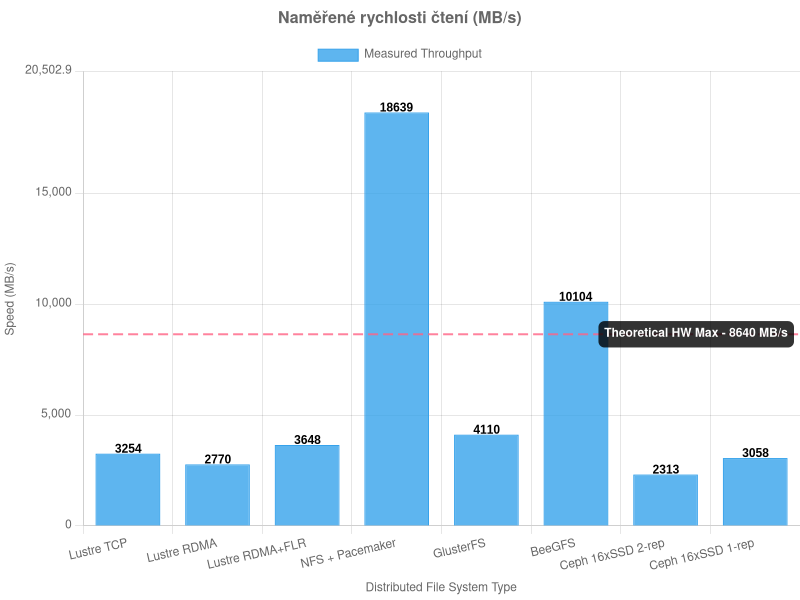
\includegraphics[width=0.65\textwidth]{assets/read_performance.png}
\end{center}
\note{
\begin{itemize}
 \item \textbf{NFS + Pacemaker} je outlier .... cache v paměti a když to bylo zakázáno v CFG
 \item \textbf{NFS + Pacemaker} NUKE + velice riskatní protože hlava dělá veškerou logiku RAID arr
 \item \textbf{BeegFS} Super výsledke ... ALE v CE je jen RAID 0 ... nelze použit v PROD
\end{itemize}
}
\end{frame}

\begin{frame}{Stav práce}{Výsledky měření - Zápis}
\begin{center}
   \vspace{-0.2cm}
   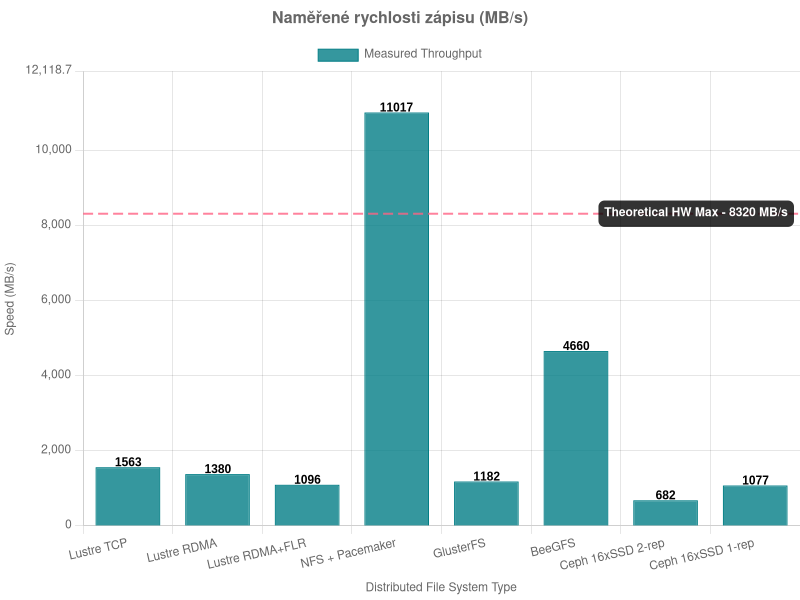
\includegraphics[width=0.65\textwidth]{assets/write_performance.png}
\end{center}
\note{
\begin{itemize}
 \item \textbf{NFS + Pacemaker} je outlier .... cache v paměti a když to bylo zakázáno v CFG
 \item \textbf{NFS + Pacemaker} NUKE + velice riskatní protože hlava dělá veškerou logiku RAID arr
 \item \textbf{BeegFS} Super výsledke ... ALE v CE je jen RAID 0 ... nelze použit v PROD
\end{itemize}
}
\end{frame}




\closingslide{Děkuji za pozornost}{Otázky?}

\end{document}
